%%%%%%%%%%%%%%%%%%%%%%%%%%%%%%%%%%%%%%%%%%%%%%
\section{Canids}
%%%%%%%%%%%%%%%%%%%%%%%%%%%%%%%%%%%%%%%%%%%%%%

\begin{frame}
\begin{figure}
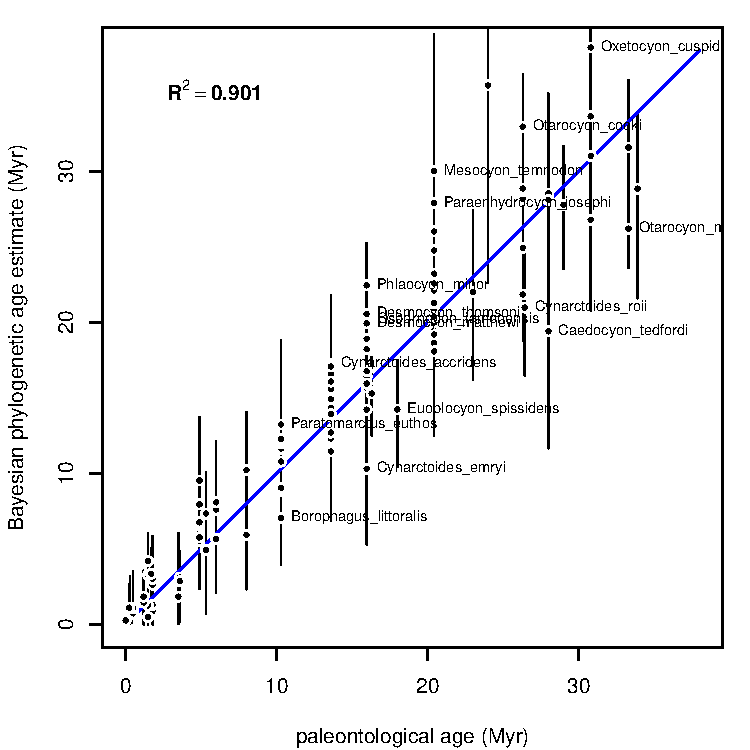
\includegraphics[width=0.70\textwidth]{../canids/1c_phyloAgeVsGeoAge.pdf}
\end{figure}
{\small Bayesian phylogenetic ages for each of 123 canid fossils plotted against palaeontological ages, under \Mstrict{}. 
Bayesian estimates are represented by the median and the 99\% HPD interval of posterior. Blue line shows the $x=y$. 
16 fossils with inconsistent estimates are labelled.}
\end{frame}

%%%%%%%%%%%%%%%%%%%%%%%%%%%%%%%%%%%%%%%%%%%%%%

\begin{frame}
\begin{figure}
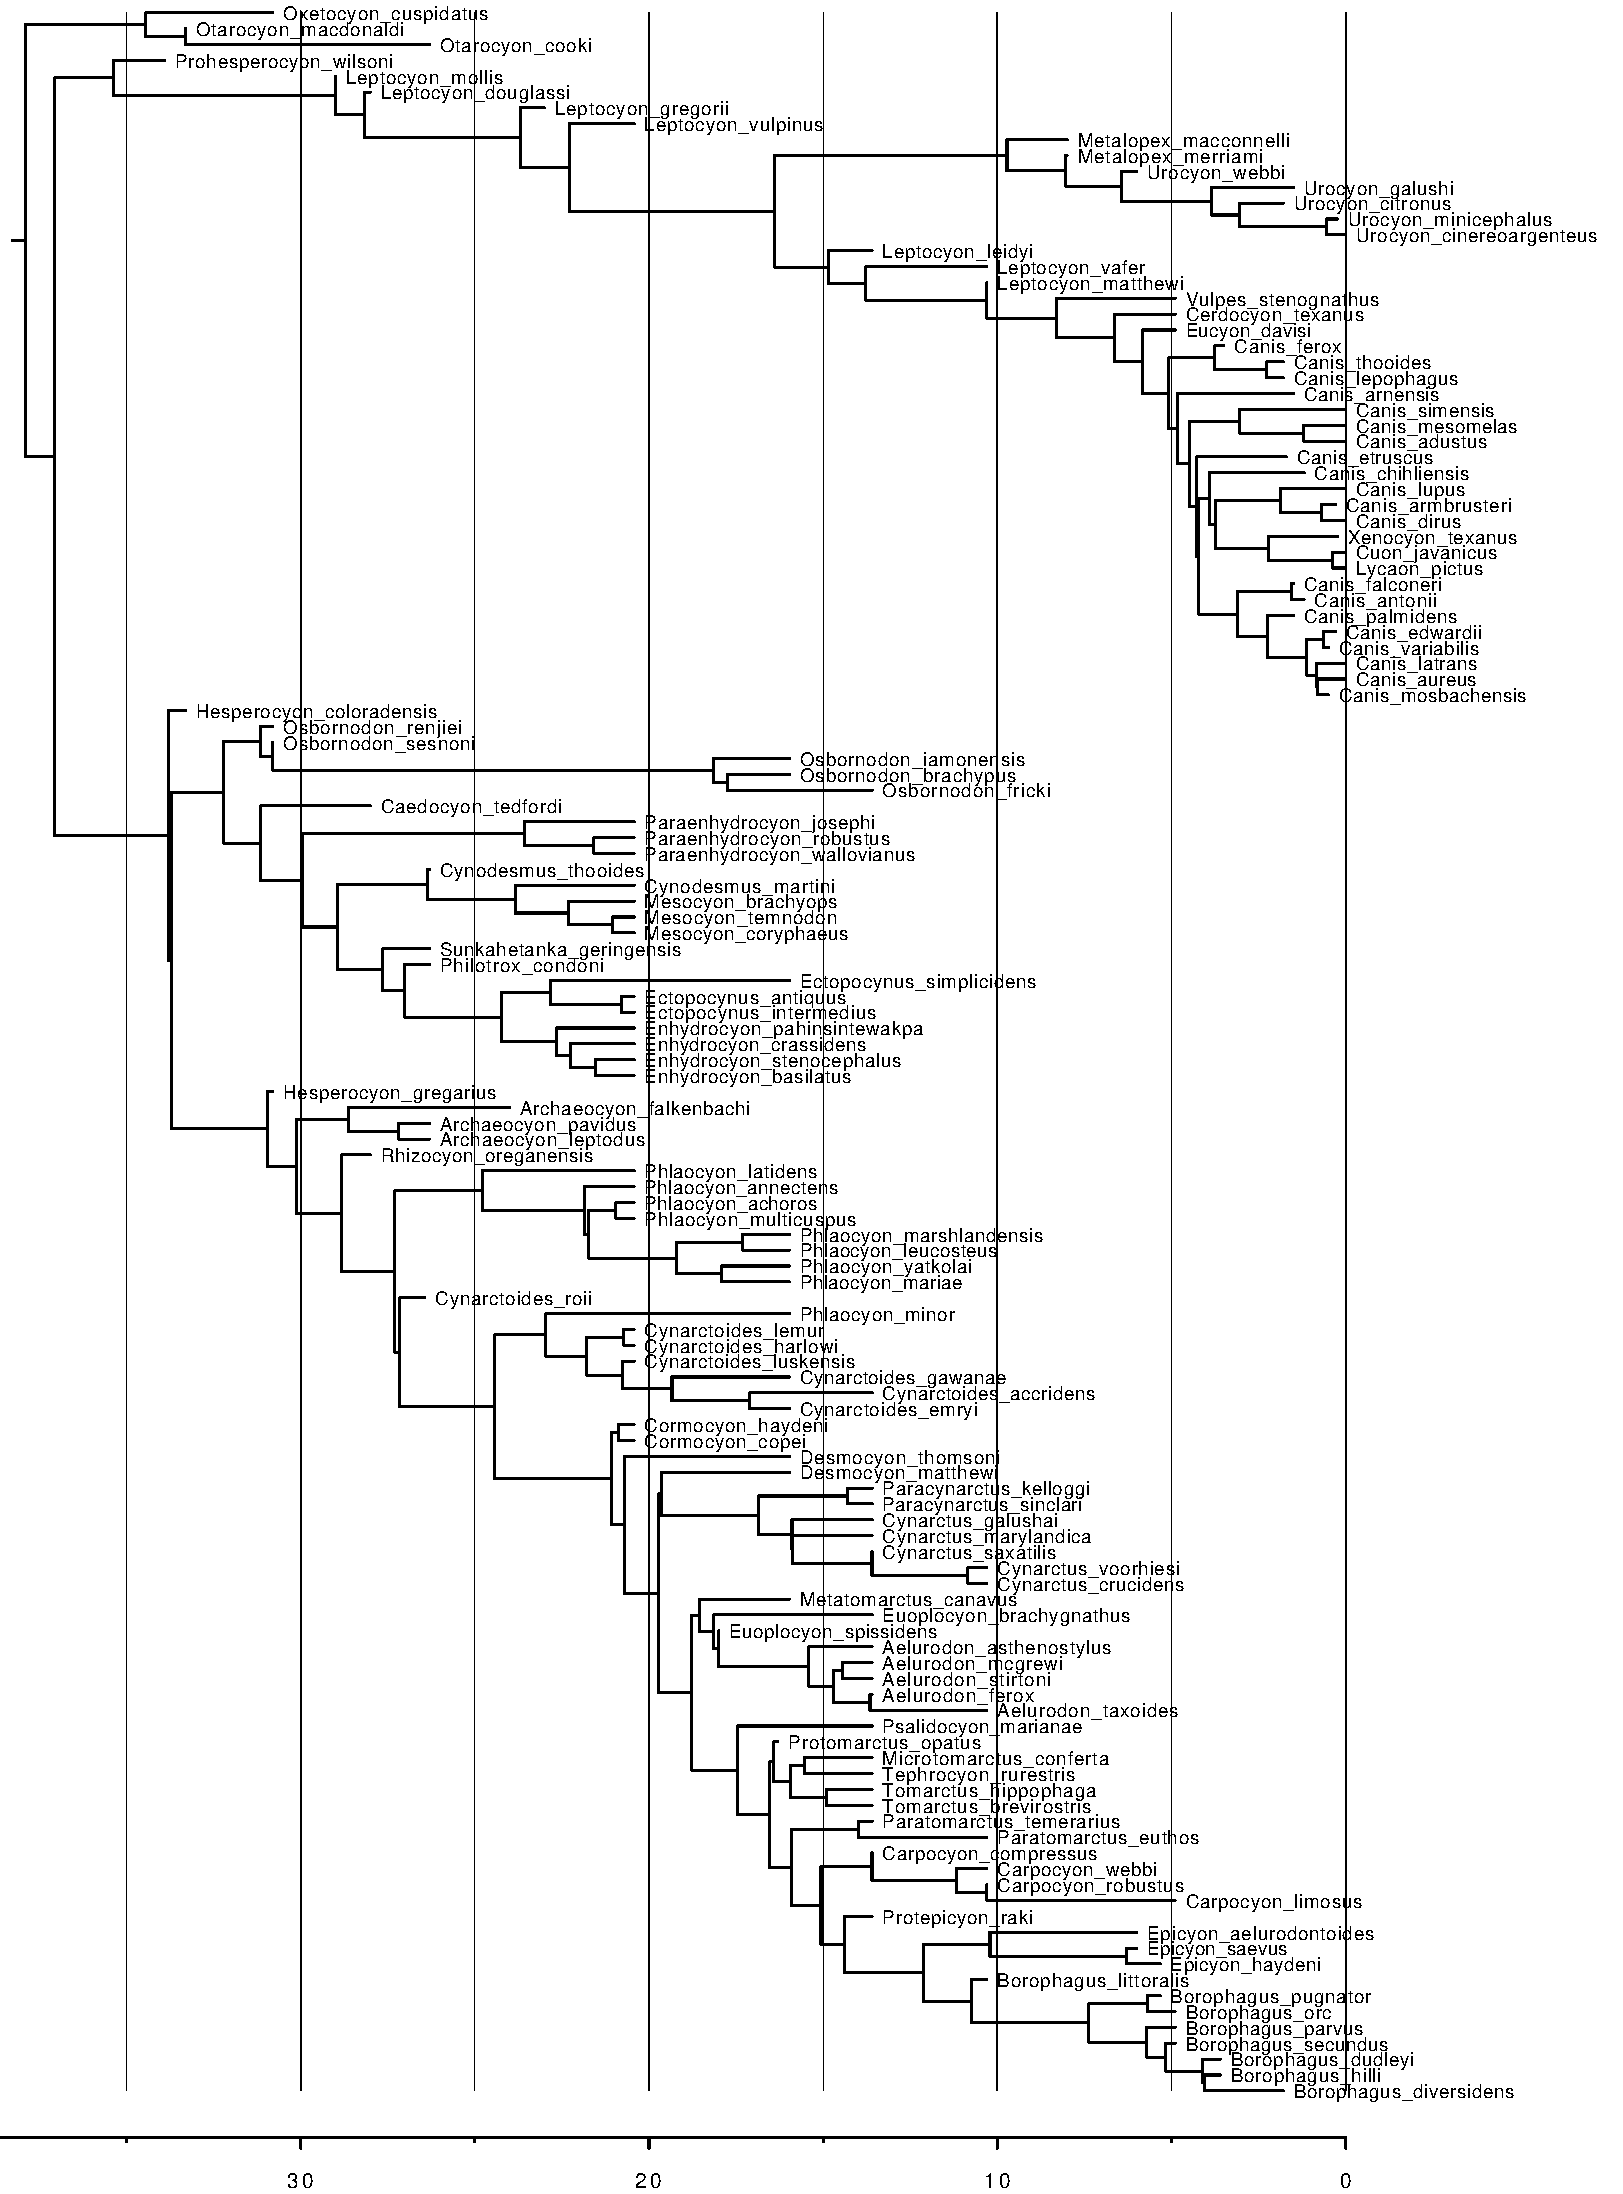
\includegraphics[width=0.5\textwidth]{../canids/1_canids-1440516016976-tree5001.pdf}
\end{figure}
A sample from the posterior distribution of an analysis of the canid data set, showing two main clades, one containing the extant taxa and another constituted entirely of extinct fossil species.
\end{frame}
